\section{Dynamic Programming algorithms}

Dynamic Programming is a problem-solving technique first introduced in the 1940s by Richard Bellman.
It focuses on finding optimal solutions by breaking problems down into overlapping subproblems, solving each once, and storing the results to avoid redundant calculations. 
The term dynamic highlights the approach's adaptability to the time-varying nature of certain problems, while programming originally referred to developing an optimized sequence of decisions, akin to a military plan or schedule for logistics or training.

\subsection{Longest Common Subsequence}
Given two sequences $x[1\dots m]$ and $y[1\dots n]$, the objective of the Longest Common Subsequence (LCS) problem is to find the longest sequence of elements that appears in both $x$ and $y$ in the same relative order.
A subsequence is derived by deleting some (or none) of the elements from a sequence without changing the order of the remaining elements. 
Thus, the LCS is the longest such sequence common to both $x$ and $y$.

\subsubsection{Naive algorithm}
A naive approach to solving the LCS problem involves generating all possible subsequences of $x$ and checking each one to see if it is also a subsequence of $y$. 
The steps for this brute-force algorithm are as follows:
\begin{enumerate}
    \item \textit{Generate all subsequences of $x$}: for a sequence of length $m$, there are $2^m$ possible subsequences. 
        Each subsequence corresponds to a unique bit vector of length $m$where each bit indicates whether the corresponding element in $x$ is included in that subsequence.
    \item \textit{Check each subsequence in $y$}: for each subsequence of $x$, verify if it also appears as a subsequence in $y$. 
        This can be done by iterating over $y$ and confirming that the elements of the subsequence appear in the same order within $y$.
    \item \textit{Track the LCS}: while iterating through all possible subsequences, keep a record of the longest one that is a subsequence of both $x$ and $y$. 
        Once all subsequences have been checked, the LCS found is the solution.
\end{enumerate}
The naive approach is highly inefficient due to its exponential time complexity.
With $m$ elements in $x$, there are $2^m$ possible subsequences, as each element has the option to be included or excluded.
Checking if a subsequence of $x$ is also a subsequence of $y$ takes $\mathcal{O}(n)$ time.
Therefore, the total time complexity for the naive algorithm is:
\[T(n)=\mathcal{O}(n2^m)\]

\subsubsection{Recursive algorithm}
To solve the LCS problem using a recursive approach, we break it down into two main steps:
\begin{enumerate}
    \item \textit{Compute the length of the LCS}: define a recursive function that calculates the length of the LCS between prefixes of two sequences, $x$ and $y$. 
    \item \textit{Extend to contruct the LCS itself}: moodify the function to also record subsequence characters, allowing reconstruction of the LCS.
\end{enumerate}
We define a two-dimensional array $c[i, j] = \left\lvert \text{LCS}(x[1 \dots i], y[1 \dots j])\right\rvert $, where each cell $c[i, j]$ represents the length of the LCS between the prefixes $x[1 \dots i]$ and $y[1 \dots j]$.
The value at $c[m,n]$ then gives the length of the LCS for the entire sequences $x$ and $y$. 
\begin{theorem}
    The recursive relation for $c[i,j]$ is given by:
    \[\begin{cases}
        c[i-1, j-1] + 1 \qquad\qquad\qquad \text{if }x[i] = y[j] \\
        \max\left\{c[i-1, j], c[i, j-1]\right\} \qquad \text{otherwise}
    \end{cases}\]
\end{theorem}
This recursive approach leverages the optimal substructure property of the LCS, meaning that the optimal solution to the LCS problem for sequences $x$ and $y$ depends on optimal solutions to subproblems involving prefixes of these sequences.
\begin{definition}[\textit{Optimal substructure}]
    An optimal solution to a problem instance includes optimal solutions to its subproblems.
\end{definition}
\begin{algorithm}[H]
    \caption{Recursive LCS}
    \begin{algorithmic}
        \Function{LCS}{$x,y,i,j$}
            \If{$x[i] = y[j]$} 
                \State $c[i,j]=\Call{LCS}{x, y, i-1, j-1} +1$
            \Else 
                \State $c[i,j]=\max\{\Call{LCS}{x, y, i-1, j},\Call{LCS}{x, y, i, j-1}\}$
            \EndIf 
            \State \Return $c[i,j]$
        \EndFunction
    \end{algorithmic}
\end{algorithm}  
In the worst-case scenario, when $x[i] \neq y[j]$, the algorithm recursively evaluates two subproblems for each pair $(i,j)$, leading to an exponential time complexity of $\mathcal{O}(2^{m+n})$.
Since many subproblems are recalculated multiple times, this recursive approach can be highly inefficient without further optimization.

\paragraph*{Memoization}
To eliminate redundant calculations, we use memoization, storing results of previously solved subproblems in a table.
When the algorithm encounters a subproblem it has solved before, it retrieves the stored result instead of recalculating it.
\begin{definition}[\textit{Memoization}] 
    Memoization is a technique where, after computing the solution to a subproblem, we store it in a table so that future calls can retrieve the result directly, avoiding redundant work.
\end{definition}
\begin{algorithm}[H]
    \caption{Memoized recursive LCS}
    \begin{algorithmic}
        \Procedure{LCS}{$x,y,i,j$}
        \If{$c[i, j] = \text{null}$}
            \If{$x[i] = y[j]$} 
                \State $c[i,j]=$ \Call{LCS}{$x, y, i-1, j-1$} $+$ 1
            \Else 
                \State $c[i,j]=\max[$\Call{LCS}{$x, y, i-1, j$},\Call{LCS}{$x, y, i, j-1$} $]$
            \EndIf 
        \EndIf
        \EndProcedure
    \end{algorithmic}
\end{algorithm}  
By storing each subproblem's solution only once, the memoization approach reduces the time complexity to $\Theta(mn)$, where $m$ and $n$ are the lengths of sequences $x$ and $y$.
This is because we compute each of the $mn$ subproblems only once.
he space complexity is also $\Theta(mn)$, as we store each subproblem result in a table.

\subsubsection{Dynamic Programming}
The Dynamic Programming approach to solving the LCS problem avoids recursion by systematically building the solution from the smallest subproblems up to the full problem.
This bottom-up approach is efficient in both time and space, eliminating the overhead of recursive calls.

The steps involved in the DP solution are as follows:
\begin{enumerate}
    \item \textit{Construct the table}: create a table $c$ where $c[i,j]$ holds the length of the LCS for prefixes $x[1\dots i]$ and $y[1\dots j]$. 
        Initialize $c[0,0]$ and fill the table up to $c[m,n]$ based on the recurrence relation used in the recursive solution.
    \item \textit{Reconstruct the LCS}: after computing $c[m,n]$, use the table to backtrack from $c[m,n]$ to $c[0,0]$, tracing the characters that contribute to the LCS.
\end{enumerate}
\begin{algorithm}[H] 
    \caption{Dynamic Programming LCS} 
    \begin{algorithmic} 
        \Procedure{LCS}{$x, y$} 
            \State Initialize $c[0\dots m,0\dots n]$ to 0 
            \For{$i = 1$ to $m$} 
                \For{$j = 1$ to $n$} 
                    \If{$x[i] = y[j]$} 
                        \State $c[i, j] = c[i-1, j-1] + 1$ 
                    \Else 
                        \State $c[i, j] = \max(c[i-1, j], c[i, j-1])$ 
                    \EndIf 
                \EndFor 
            \EndFor 
            \State \Return $c[m, n]$ 
        \EndProcedure 
    \end{algorithmic} 
\end{algorithm}
This approach has a time complexity of $\mathcal{O}(mn)$ as each entry of the $m\times n$ table is filled once.
The space complexity is also $\mathcal{O}(mn)$, since we store each subproblem result in the table.
This Dynamic Programming method is both efficient and avoids redundant calculations, making it well-suited for large inputs.

\subsection{Binary Decision Diagram}
Binary Decision Diagrams (BDDs) are a compact data structure for representing Boolean functions.
They improve on traditional approaches by storing evaluated sub-cases in memory, allowing for efficient retrieval and manipulation of Boolean expressions. 
BDDs are particularly valuable because they can be made canonical, which provides a unique representation for each Boolean function with a fixed variable ordering, enabling easier comparison and optimization.

One of the key benefits of BDDs is their efficiency in performing Boolean operations, such as conjunction, disjunction, and negation. 
However, the size of a BDD heavily depends on the chosen variable ordering; optimal ordering can significantly reduce the size and complexity of the BDD.

In a BDD, a Boolean function is represented as a Directed Acyclic Graph (DAG) with: single root node representing the function's entry point and two terminal nodes labeled $0$ and $1$, representing the function's output values.
Each internal node is associated with a variable and has exactly two children, representing the function's behavior when that variable is assigned $1$ or $0$.

\paragraph*{Ordered BDD}
An Ordered BDD (OBDD) applies only the ordering constraint, requiring that variables appear in a specific sequence along any path but without enforcing reduction.

\paragraph*{Reduced Ordered BDD}
An ROBDD is a special type of BDD that is both reduced and ordered, resulting in a compact, canonical representation for Boolean functions.
An ROBDD is derived from a Shannon co-factoring tree with two main modifications:
\begin{itemize}
    \item \textit{Reduction}: this process eliminates redundancy by: 
        \begin{itemize}
            \item Removing nodes with identical children.
            \item Merging nodes with identical subgraphs, so that each unique subgraph appears only once in the diagram.
        \end{itemize}
    \item \textit{Ordering}: variables are processed in a fixed, consistent order along every path from the root to a terminal node. 
        This ordering ensures that each path encounters variables in a predefined sequence, contributing to the canonical nature of ROBDDs.
\end{itemize}
The canonical structure of an ROBDD allows straightforward identification of the function's onset (the set of variable assignments that make the function evaluate to $1$). 
This can be achieved by tracing all paths from the root to the $1$-terminal node. 
Each such path represents a set of variable assignments that satisfy the Boolean function.

\subsubsection{Implementation}
The efficient implementation of BDDs relies on specific data structures that prevent redundancy, streamline Boolean operations, and optimize memory usage. 
The key components are:
\begin{itemize}
    \item \textit{Unique table}: ensures that each node in the BDD is unique, preventing duplication. 
        This is typically implemented as a hash table, where the properties of each node serve as a key mapping to a unique existing or newly created node.
    \item \textit{Computed table}: stores the results of previously computed operations to speed up repeated calculations.
        This table, which can be implemented as a hash table, indexes operations in the form $(f,g,h)$, representing arguments passed to the ITE operator. 
        If a result for $(f,g,h)$ exists in the table, it can be retrieved without recomputation.
\end{itemize}

\paragraph*{ITE operator}
The ITE operator is central to BDD operations, as it can implement any binary Boolean function. 
Mathematically, the ITE operator is defined as:
\[\text{ite}(f,g,h)=fg+f\bar{h}\]
Before adding a new node $(v, g, h)$ is added to the BDD, the unique table is checked to avoid duplication. 
If a matching node exists, its pointer is reused; otherwise, a new node is created and added to the unique table.
\begin{algorithm}[H]
    \caption{Recursive ITE}
    \begin{algorithmic}
        \Function{ITE}{$f, g, h$}
            \If{$f = 1$} 
                \State \Return $g$
            \EndIf
            \If{$f = 0$} 
                \State \Return $h$
            \EndIf
            \If{$g = h$} 
                \State \Return $g$
            \EndIf
            \If{$p = \Call{HashLookupComputedTable}{f, g, h}$} 
                \State \Return $p$
            \EndIf
            \State $v = \Call{TopVariable}{f,g,h}$
            \State $f_n = \Call{ITE}{f_v, g_v, h_v}$
            \State $g_n = \Call{ITE}{f_{\bar{v}}, g_{\bar{v}}, h_{\bar{v}}}$
            \If{$f_n = g_n$} 
                \State \Return $g_n$
            \EndIf
            \If{$!(p = \Call{HashLookupComputedTable}{v, f_n, g_n})$}
                \State $p=$ \Call{CreateNode}{$v, f_n, g_n$}
                \State Insert $p$ into the unique table
            \EndIf
            \State $key= \Call{HashKey}{f, g, h}$
            \State \Call{InsertComputedTable}{$p,key$}
            \State \Return $p$
        \EndFunction
    \end{algorithmic}
\end{algorithm}

\paragraph*{Complemented edges}
Complemented edges optimize memory and operation efficiency by allowing the BDD to represent negated functions without additional nodes.
This technique reduces storage needs and accelerates NOT and ITE operations.
To maintain the canonical form of the BDD, certain edge equivalences are managed, ensuring consistent representation across nodes.
\begin{figure}[H]
    \centering
    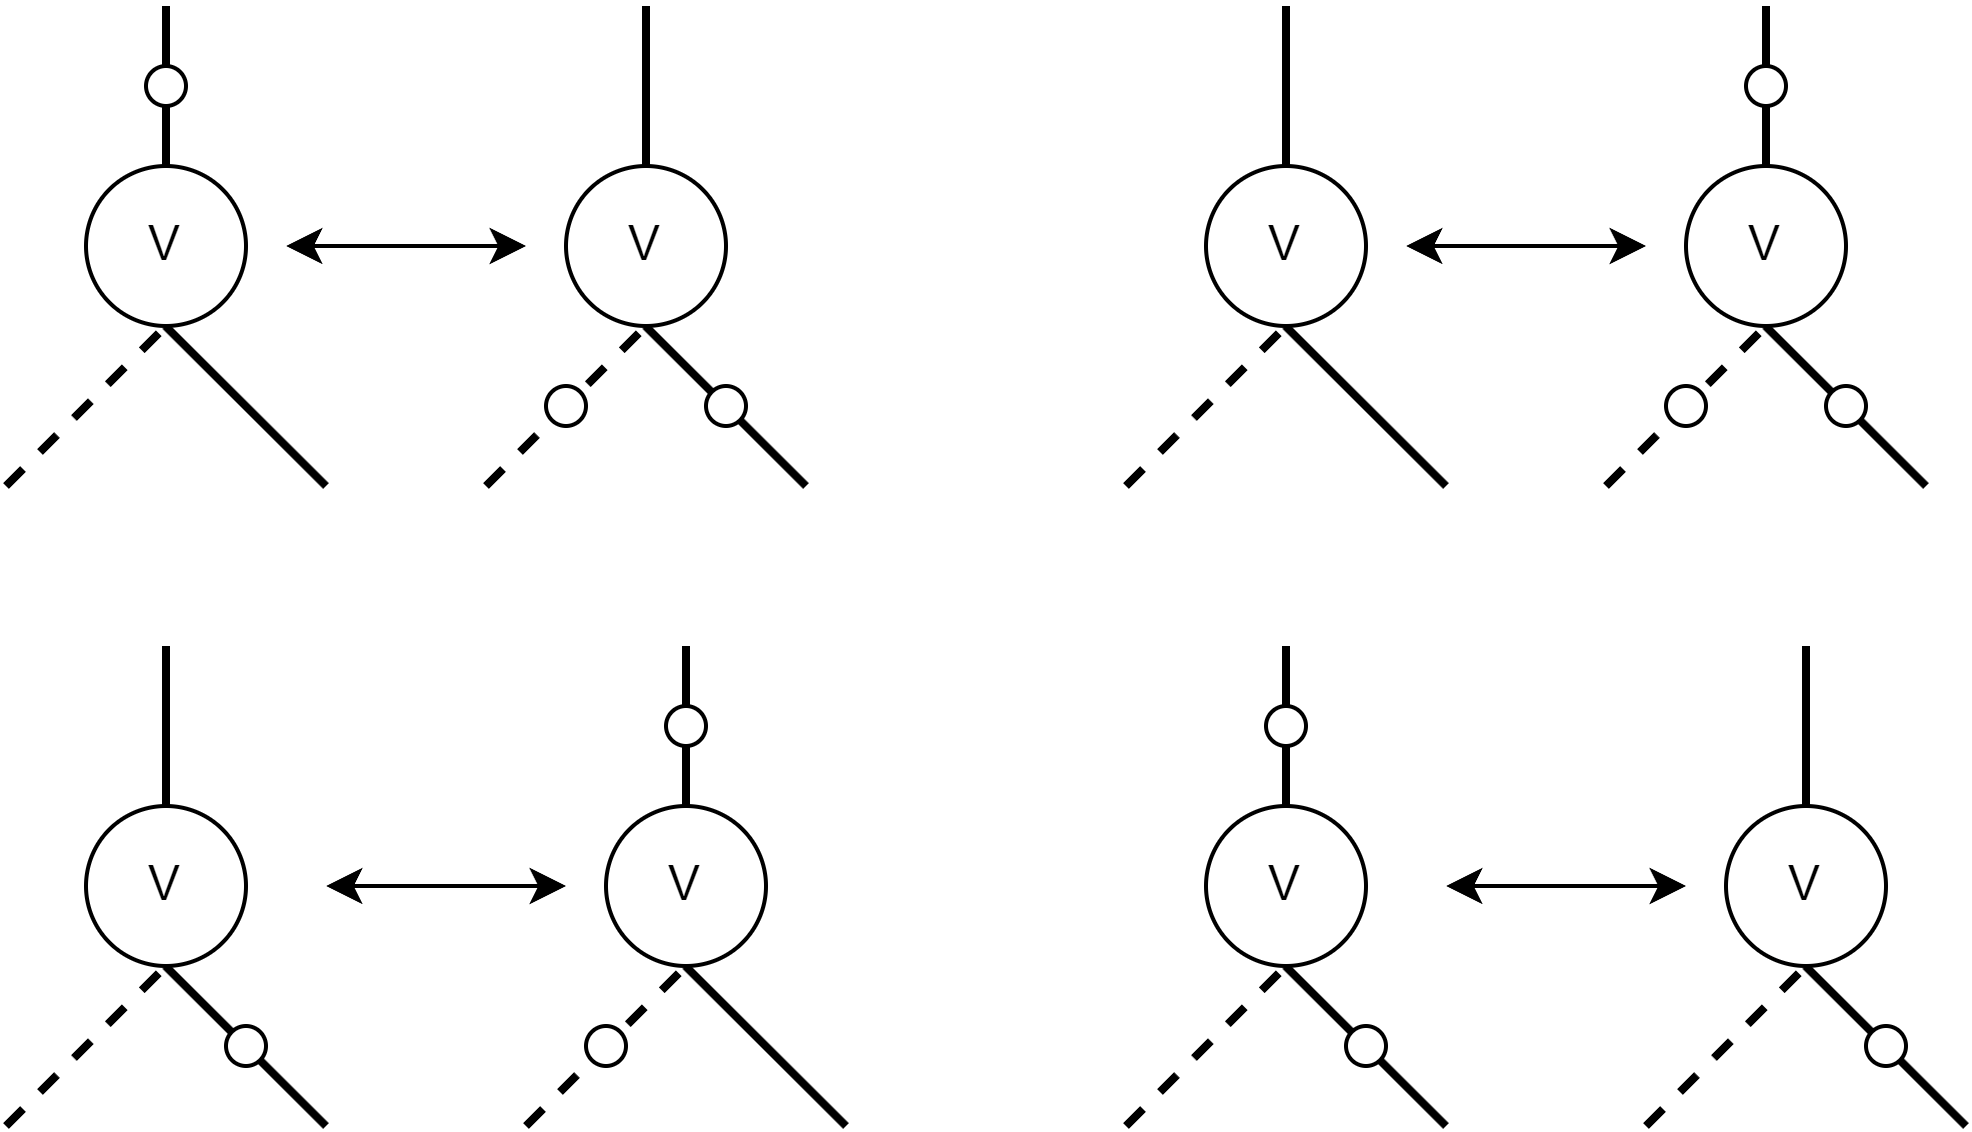
\includegraphics[width=0.75\linewidth]{images/ed1.png}
    \caption{Edge equivalence}
\end{figure}

\paragraph*{Optimization}
To maximize matches in the computed table, conventions are applied, such as selecting the argument with the smallest top variable (or smallest pointer in case of a tie) as the first argument. 
Caching mechanisms—including local caching, operation (specific caching, and shared caching) also contribute to efficient BDD operations.

\subsubsection{Garbage collection}
Effective garbage collection is essential for managing memory usage in BDDs, as unreferenced nodes consume resources and degrade performance. 
Garbage collection in BDDs typically involves:
\begin{enumerate}
    \item \textit{Reference counting}: each node tracks the number of references to it, allowing immediate deallocation when the reference count drops to zero.
    \item \textit{Mark-and-sweep}: this process involves marking nodes with references during a traversal and then sweeping through to delete unmarked nodes in a second pass.
\end{enumerate}
Garbage collection timing is important to optimize resource usage without excessive overhead. 
Nodes can be deallocated on demand, at specific intervals, or after predefined operations. 
Since computed tables do not track references, they are cleared separately during the garbage collection process to maintain efficiency.